% !TEX root =  ../main_manuscript.tex

\section{Results}
\label{sec:results}
We first discuss the results pertaining to the joint model fitted to the PRIAS dataset and then discuss results from the simulation study.
\subsection{Model Fit}
From the joint model fitted to the PRIAS dataset, we found that both $\log_2 \{\mbox{PSA} + 1\}$ velocity,  and log odds of having $\mbox{DRE} > \mbox{T1c}$  were significantly associated with the hazard of cancer progression. For any patient, an increase in $\log_2 \{\mbox{PSA} + 1\}$ velocity from −0.03 to 0.16 (first and third quartiles of the fitted velocities, respectively) corresponds to a 1.92 fold increase in the hazard of cancer progression. Whereas, an increase in log odds of $\mbox{DRE} > \mbox{T1c}$ from -6.65 to -4.36 (first and third quartiles of the fitted log odds, respectively) corresponds to a 1.40 fold increase in the hazard of cancer progression. In terms of the predictive performance, we found that the area under the receiver operating characteristic curves (AUC) \cite{landmarking2017} was 0.65, 0.62, 0.75, 0.71 and 0.59 at years one, two, three, four, and five of follow‐up, respectively. Parameter estimates are presented in detail in Appendix B of the supplementary material.

\subsection{Simulation Study}
Figure \ref{fig:mean_nb_offset} shows the mean (obtained from 500 x 250 test patients) number of biopsies conducted by various biopsy schedules, plotted against the corresponding delay in detection of cancer progression in years (time of last biopsy - true time of cancer progression). The general trend is that more biopsies are required to have a smaller delay in detection.

\begin{figure}[!htb]
\captionsetup{justification=justified}
\centerline{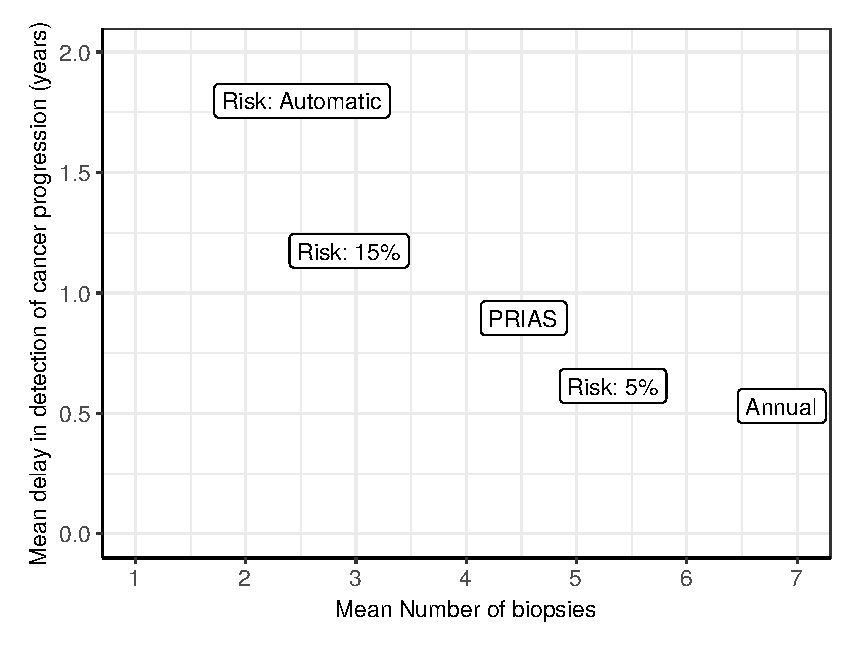
\includegraphics[width=\columnwidth]{images/mean_nb_offset.eps}}
\caption{Mean number of biopsies (of 500 x 250 test patients) scheduled by various biopsy schedules, plotted against the corresponding delay in detection of cancer progression, in years (time of last biopsy - true time of cancer progression). Biopsies are conducted until cancer progression is detected. \textbf{Types of personalized schedules:} Risk:~15\% and Risk:~5\% approaches, schedule biopsy if the risk of cancer progression at a visit is more than 15\% and 5\%, respectively. Risk:~Automatic works similar to Risk:~15\% and Risk:~5\%, except that the risk threshold for biopsy is chosen automatically by maximizing $\mbox{F}_1$ score (see \hyperref[sec:methods]{Methods}). Annual corresponds to a schedule of yearly biopsies and PRIAS corresponds to biopsies as per PRIAS protocol (see \hyperref[sec:introduction]{Introduction}).}
\label{fig:mean_nb_offset}
\end{figure}

Since patients have varying cancer progression speeds, the impact of different approaches for biopsies also varies with the speed. In order to highlight these differences we trichotomize patients into 3 categories (fast, intermediate, slow speed) as per their time of cancer progression. In the simulated patients, we observed that for roughly 50\% of the patients cancer progression did not take place in the 10 year follow-up. These could be seen as patients with a slow speed of cancer progression. Roughly 30\% of the patients obtain cancer progression within first 3.5 years. These could be high risk patients who choose AS instead of immediate treatment, or patients with an initially misdiagnosed state of cancer \cite{cooperberg2011outcomes}. These patients can be considered as fast progressing patients. We consider that the remaining 20\% patients with cancer progression times between 3.5 and 10 years have an intermediate speed of cancer progression. Although such a trichotomization may not be perfect and can only be done retrospectively in a simulation setting, we do it only for the purpose of illustration.

\begin{figure}[!htb]
\captionsetup{justification=justified}
\centerline{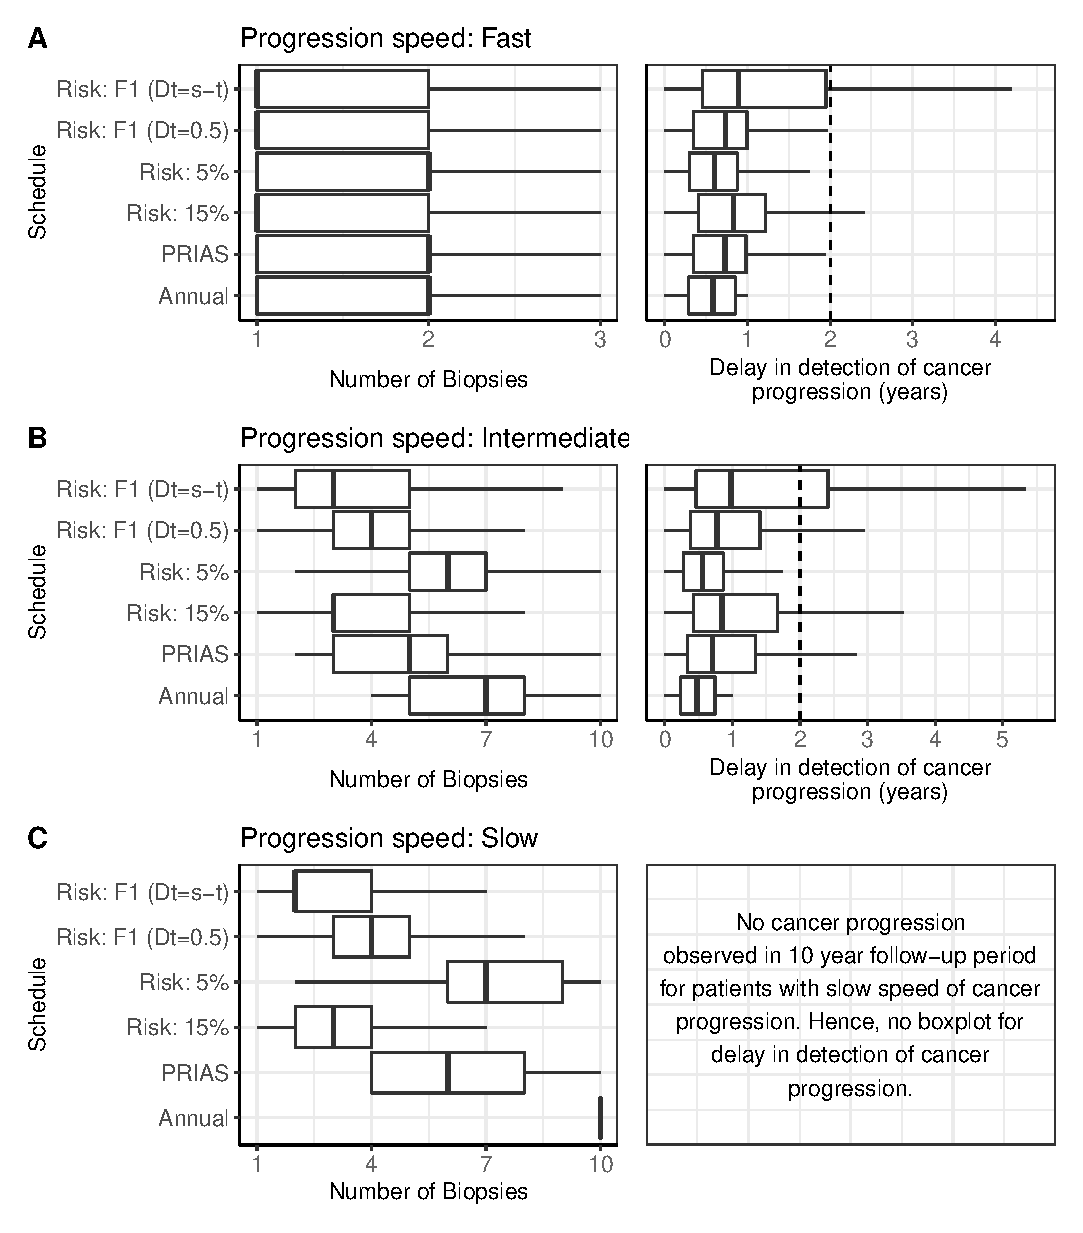
\includegraphics[width=\columnwidth]{images/sim_res_combined.eps}}
\caption{Boxplot showing variation in number of biopsies, and the delay in detection of cancer progression, in years (time of last biopsy - true time of cancer progression) for various biopsy schedules. Biopsies are conducted until cancer progression is detected. \textbf{Panel~A:} results for simulated patients who had a faster speed of cancer progression, with progression times between 0 and 3.5 years. \textbf{Panel~B:} results for simulated patients who had an intermediate speed of cancer progression, with progression times between 3.5 and 10 years. \textbf{Panel~C:} results for simulated patients who did not have cancer progression in the 10 years of follow-up. \textbf{Types of personalized schedules:} Risk:~15\% and Risk:~5\% approaches, schedule biopsy if the risk of cancer progression at a visit is more than 15\% and 5\%, respectively. Risk:~Automatic works similar to Risk:~15\% and Risk:~5\%, except that the risk threshold for biopsy is chosen automatically by maximizing $\mbox{F}_1$ score (see \hyperref[sec:methods]{Methods}). Annual corresponds to a schedule of yearly biopsies and PRIAS corresponds to biopsies as per PRIAS protocol (see \hyperref[sec:introduction]{Introduction}).}
\label{fig:sim_res_combined}
\end{figure}

For faster progressing patients (30\% of the total patients), the boxplots in panel A of Figure~\ref{fig:sim_res_combined} shows the variation in the number of biopsies (of 500 x 250 test patients), and the delay in detection of cancer progression, in years (time of last biopsy - true time of cancer progression) due to various biopsy schedules. We can see that the personalized schedules conduct a median of one biopsy compared to two biopsies for PRIAS and annual schedule. The performance of personalized schedule with 15\% risk threshold is similar to that of PRIAS schedule. Thus with personalized approach, one biopsy may get saved for faster progressing patients.

For patients with intermediate progression speed (20\% of the total patients), the boxplots in panel B of Figure~\ref{fig:sim_res_combined} shows the variation in number of biopsies, and the delay in detection of cancer progression due to various biopsy schedules. Firstly, we can see that personalized schedules with a small risk threshold such as 5\% risk conduct many more biopsies than other personalized schedules. Consequently, their performance with respect to the delay in detection of progression is similar to that of annual schedule. However, personalized schedule with slightly higher risk (15\%) and risk chosen automatically, schedule a median of 3 biopsies each. This is despite the fact that the delay in detection of cancer progression due to the schedule with 15\% risk threshold is similar to that of the PRIAS schedule. However, the PRIAS schedule conducts more biopsies (median of 5 biopsies). Thus, the personalized approach may lead to two less biopsies for patients with intermediate speed of progression.

The patients who are at most advantage with the personalized schedules are the patients who progress slowly (50\% of the total patients). Panel C of Figure~\ref{fig:sim_res_combined} shows a boxplot of the number of biopsies conducted by various biopsy schedules for such patients. It can be seen that the annual schedule may lead to 10 unnecessary biopsies for everyone. The PRIAS schedule, schedules a median of 6 unnecessary biopsies. In comparison the personalized schedules using 15\% risk threshold and automatically chosen risk threshold, schedule only 2 and 3 biopsies, respectively.
